\newpage
\subsection{Creazione di un Biglietto}

	\begin{figure}[htbp]
		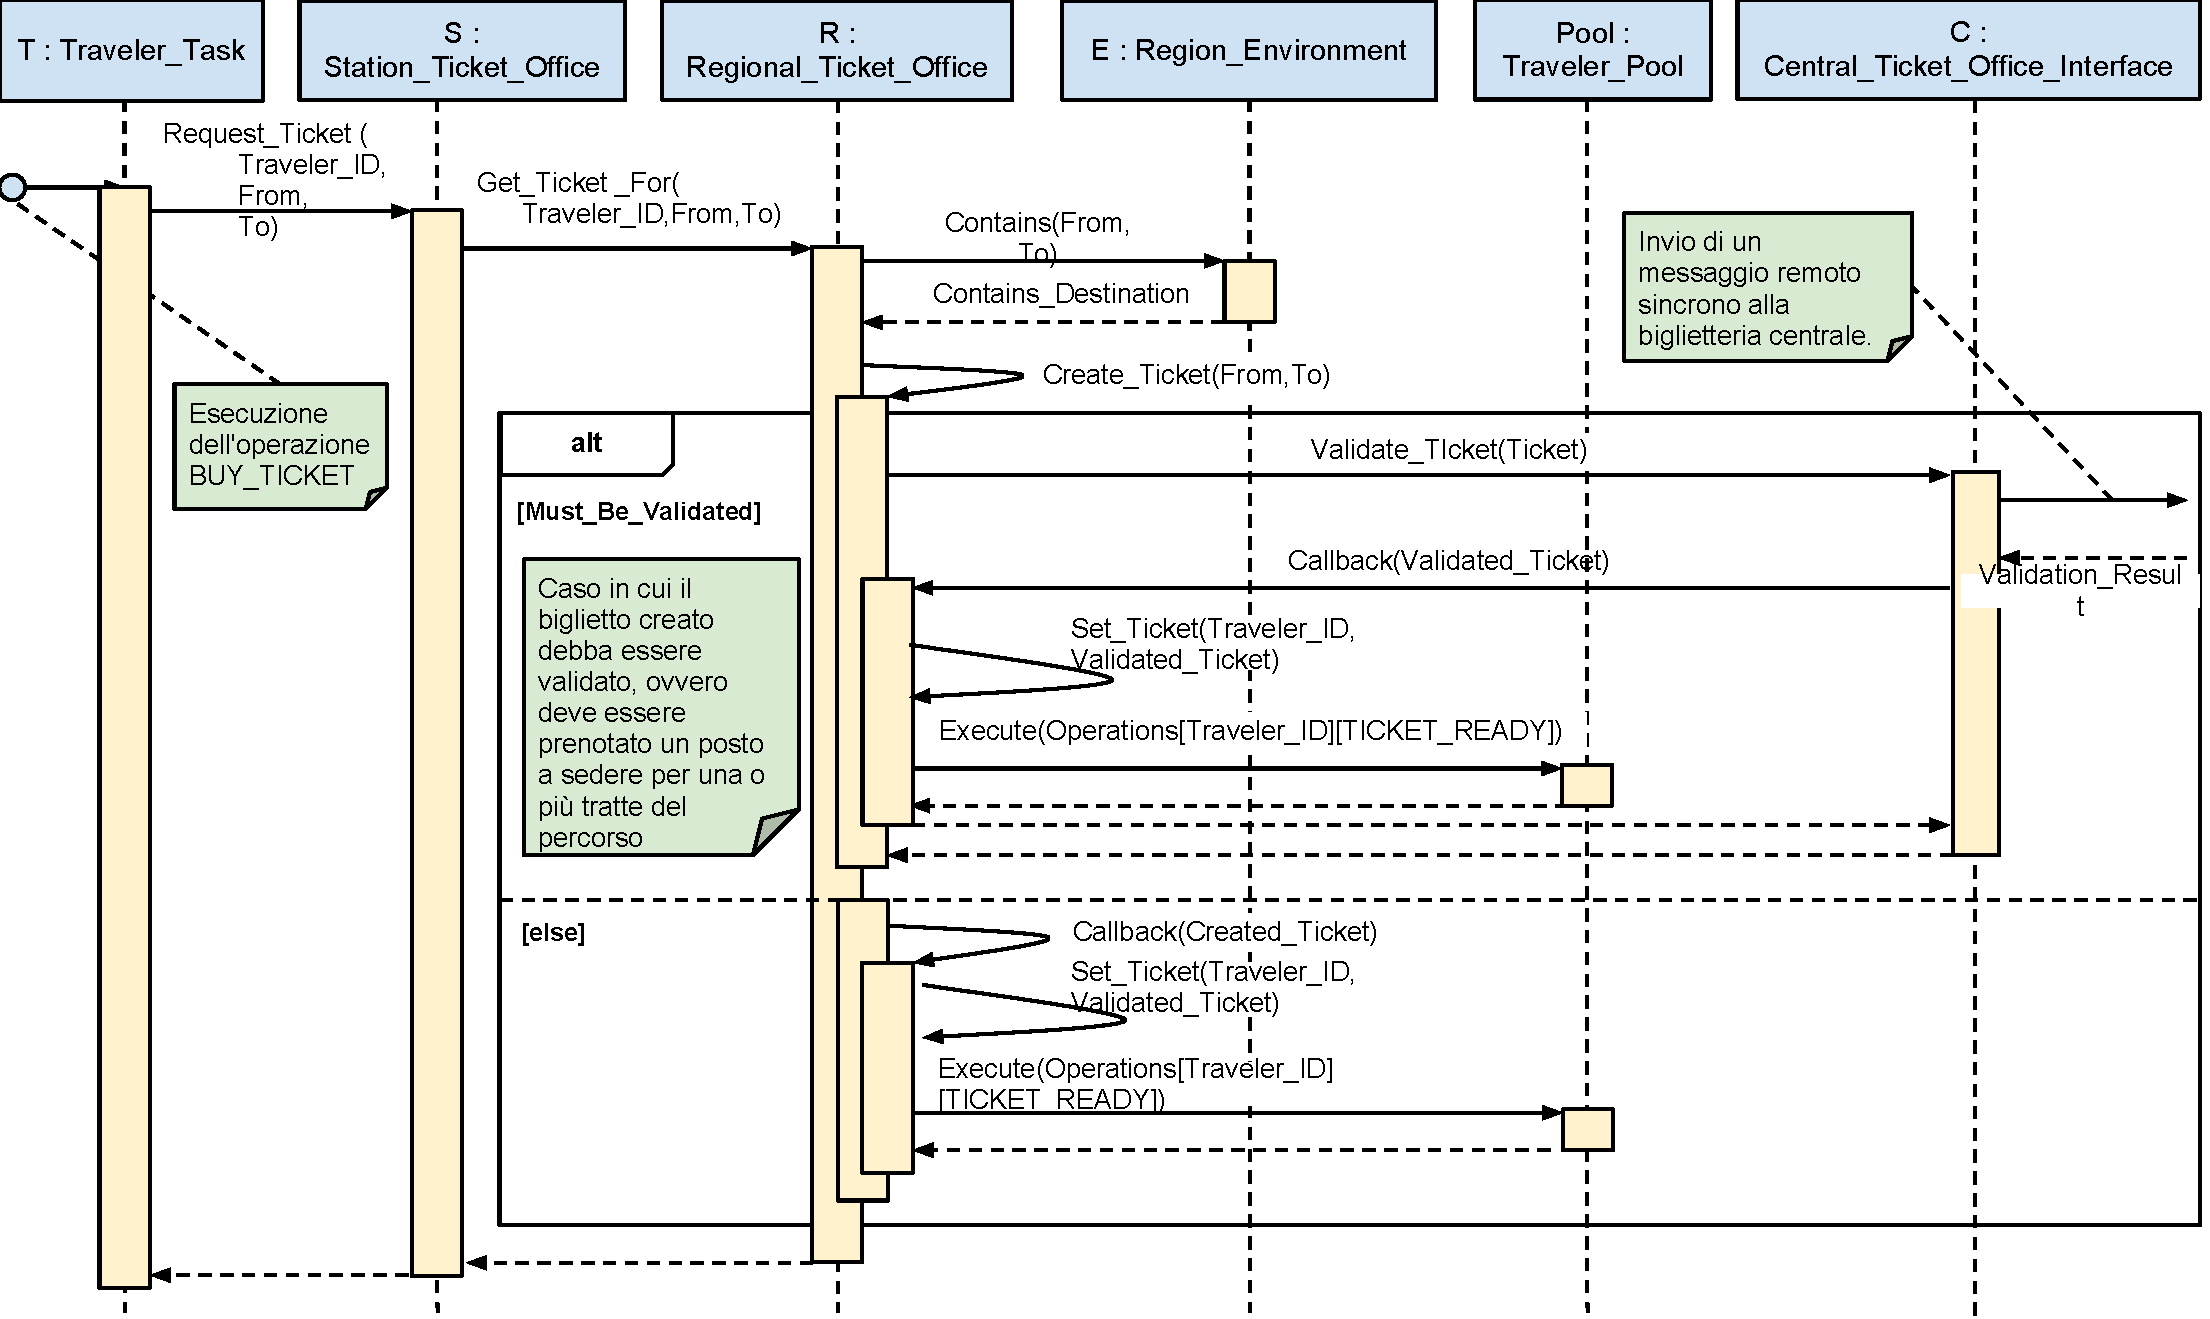
\includegraphics[trim = 55mm 0mm 0mm 0mm,scale=0.43]{imgs/Buy_Ticket_Sequence_Diagram.pdf}
		\caption{\footnotesize{Diagramma di Sequenza, operazioni necessarie alla creazione di un Ticket.}}
		\label{fig:ticket_creation_diagram}
	\end{figure}

Per la creazione di un Biglietto, necessario per permettere ai Viaggiatori di poter raggiungere una destinazione, ho utilizzato un algoritmo che coinvolge le componenti (distribuite) introdotte in sezione \ref{subsec:ticket_offices}.
Il diagramma di Sequenza in figura \ref{fig:ticket_creation_diagram} fornisce una rappresentazione delle fasi successive di creazione.

%Per richiedere la creazione di un Biglietto, ho introdotto un tipo di operazione per le entità viaggiatori, che indicherò con \ttt{CREATE\_TICKET}, mentre per gestire l'avvenuta creazione e ottenimento del Biglietto un'operazione che indicherò con \ttt{TICKET\_READY}. Quest'ultima operazione è necessaria poiché l'algoritmo ha una natura asincrona.

La descrizione sarà suddivisa in fasi sucessive:

	\subsubsection {Richiesta di Creazione}\label{subsubsec:ticket_creation_request}
	
	La richiesta di creazione di un \ttt{Ticket} da parte di un Viaggiatore, viene operata da un thread appartenente al pool di \ttt{Traveler\_Pool} che esegue l'operazione \ttt{CREATE\_TICKET} (come descritto precedentemente in sezione \ref{subsubsec:buy_ticket}). Tale operazione, effettua una richiesta di creazione alla stazione di partenza $S$, la quale inoltrerà la richiesta alla pripria Biglietteria interna. Quest'ultima richiederà la creazione effettiva alla Biglietteria Regionale, se lo stesso \ttt{Ticket} non è presente in una cache locale.  
	
	\subsubsection {Creazione del Ticket} \label{subsubsec:ticket_creation}
	
	Siano \ttt{From} e \ttt{To} rispettivamente l'identificativo della Stazione di partenza, e l'identificativo della Stazione di destinazione. Le operazioni svolte dalla procedura invocata presso la Stazione Regionale sono le seguenti:
	\begin{itemize}
		\item Se \ttt{To} appartiene alla Regione corrente, viene creato il \ttt{Ticket}, effettuando le seguenti operazioni:
			\begin {itemize}
					
				\item Si considera il percorso più breve da \ttt{From} a \ttt{To}, che indicheremo con $Path = \{s_1,...,s_N\}$. Questo percorso è ottenuto applicando un semplice algoritmo di cammino minimo sul grafo avente come veritici le Stazioni, e come archi non direzionati i Segmenti che li collegano. Il cammino può minimizzare la lunghezza totale del percorso.
				
				\item Il percorso $Path$ viene intersecato con i Percorsi dei Treni (\ttt{Route}), per poter definire le Tappe che compongono il Biglietto. Sia $i=1$, allora finché $i<=N$:
					\begin{itemize}
						\item Ottieni i percorsi dei Treni (\ttt{Route}s) $R={r_1,...,r_k}$ che contengono una Tappa $t$ tale per cui i campi \ttt{Start\_Station} e \ttt{Next\_Station} sono rispettivamente $s_i$ e $s_{i+1}$. Per ciascuno di questi percorsi, vengono ottenuti indice e posizione della tappa $t$ al suo interni.
						A qusto punto si procede all'individuazione del percorso che meglio si adatta al cammino minimo da segire. Sia quindi $k = i$; per ciascuna route $r_j \in R$, a partire dalla posizione di $t$ in $r_j$, si procede ad estendere la corrispondenza. Viene quindi mantenuto il percorso con la corrispondenza di lunghezza massima $Max\_Length$, memorizzandone l'indice in $Max\_Match$.
						\item Viene quindi creata una Tappa del \ttt{Ticket}:
						\begin{verbatim}
							- start_station        : indice della stazione 
							                         di inizio dell'estensione,
							- next_station         : indice della stazione di
							                         fine dell'estensione 
							                         massima,
							- train_id             : indice del Treno che 
							                         percorre il percorso di 
							                         indice Max_Match,
							- start_platform       : indice della Piattaforma
							                         di partenza in t,
							- destination_platform : indice della Piattaforma 
							                         dell'ultima tappa
							- next_region          : regione corrente,
							
						\end{verbatim}
						\item $i$ viene incrementato di $Max\_Length$.
					\end{itemize} 
			\item Il \ttt{Ticket} creato viene assegnato al Viaggiatore e viene quindi inserita l'operazione \ttt{TICKET\_READY} nella coda di operazioni di \ttt{Traveler\_Pool}.
			\end {itemize} 
		\item Se \ttt{To} non appartiene alla Regione corrente, allora viene effettuata una richiesta remota alla Biglietteria Centrale. Tale richiesta è asincrona, in modo tale da permettere al thread che sta effettuando la richiesta di creazione del Biglietto di non effettuare attesa attiva, e quindi di poter eseguire altre operazioni eventualmente presenti nella coda di \ttt{Traveler\_Pool}.
	\end{itemize} 


	\subsubsection {Richiesta di Creazione Remota}
	
	Una volta che la Biglietteria Centrale riceve, tramite l'interfaccia remota esposta, un messaggio remoto di richiesta di Creazione di un Biglietto, essa effettua 3 operazioni:
	\begin{itemize}
		\item Individua la Regione di appartenenza della destinazione $To$; se tale informazione non è presente nella cache locale mantenuta dalla Biglietteria Centrale, essa viene ricercata nel modo seguente: 
			\begin{itemize}
				\item viene recuperato l'elenco completo delle Regioni (ovvero una lista di coppie \ttt{(Node\_Name,Node\_Address)}) dal \ii{Server dei Nomi};
				\item per ciascun elemento dell'elenco, viene inviata una richiesta remota, alla quale ciascuna Regione risponde con \ttt{True}, se contiene la Stazione, o \ttt{False} in caso contrario.
			\end{itemize}
		\item Se nessuna risposta positiva viene ricevuta, allora viene comunicato l'errore alla Biglietteria Regionale richiedente, inviando un messaggio di errore.
		\item Nel caso in cui si abbia una risposta positiva da una Regione $R$ allora:
			\begin{itemize}
				\item Viene recuperata la lista di Regioni attraverso le quali costruire il percorso per raggiungere la destinazione (dalla mappa \ttt{Links}). 
				\item A ciascuna stazione di questa lista viene inviata una richiesta remota \ii{sincrona} per ottenere dei Ticket che collegati, permettono di raggiungere \ttt{To} a partire da \ttt{From}.
				\item I vari \ttt{Ticket} ottenuti vengono poi uniti (eliminati i passaggi per le stazioni di gateway se non necessari) e il Biglietto risultante inviato come risposta al Nodo richiedente, presso il quale verrà assegnato al viaggiatore richiedente, e verrà inserita l'operazione \ttt{TICKET\_READY} nella coda di \ttt{Traveler\_Pool}.
			\end{itemize}
	\end{itemize}
	
	\subsubsection {Validazione di un Ticket}
	
	Una volta che un Biglietto è stato 
